\documentclass[11pt,a4paper]{article}

\usepackage[utf8]{inputenc}
\usepackage[T1]{fontenc}
\usepackage{helvet}
\renewcommand{\familydefault}{\sfdefault}
\usepackage[margin=2.2cm]{geometry}
\usepackage{microtype}
\usepackage{xcolor}
\usepackage{graphicx}
\usepackage{float}
\usepackage{booktabs}
\usepackage{tabularx}
\usepackage{array}
\usepackage{enumitem}
\usepackage{titlesec}
\usepackage{tikz}
\usetikzlibrary{arrows.meta,positioning,calc}
\usepackage{listings}
\usepackage[most]{tcolorbox}
\usepackage{amsmath}
\usepackage{needspace}
\usepackage{caption}
\usepackage[colorlinks=true,urlcolor=blue!60!black,linkcolor=black]{hyperref}

\definecolor{rule}{HTML}{D0D7DE}
\definecolor{codebg}{HTML}{F6F8FA}
\definecolor{accent}{HTML}{CF222E}

\setlength{\parindent}{0pt}
\setlength{\parskip}{6pt}
\renewcommand{\arraystretch}{1.3}
\setlist{itemsep=2pt,topsep=4pt}

\titleformat{\section}{\Large\bfseries}{}{0pt}{}[\vspace{-4pt}{\color{rule}\titlerule}]
\titlespacing*{\section}{0pt}{16pt}{8pt}

\captionsetup{labelformat=empty,font=bf,justification=raggedright,singlelinecheck=false,skip=4pt}

\makeatletter
\let\oldsection\section
\renewcommand\section{\needspace{9\baselineskip}\oldsection}
\makeatother
\newcommand{\code}[1]{\texttt{\small #1}}

\lstset{basicstyle=\ttfamily\small,backgroundcolor=\color{codebg},frame=none,
  breaklines=true,columns=fullflexible,xleftmargin=6pt,xrightmargin=6pt,
  aboveskip=6pt,belowskip=6pt}

\newcommand{\shot}[2]{%
  \begin{figure}[H]
    \centering
    \captionsetup{type=figure}
    \caption*{#2}
    \fbox{\includegraphics[width=0.94\linewidth]{figures/#1}}
  \end{figure}}

\begin{document}
\pagestyle{plain}

{\fontsize{26}{30}\selectfont\bfseries Meridian --- Project Report\par}
\vspace{6pt}

\begin{tcolorbox}[enhanced,colback=blue!4,colframe=blue!4,boxrule=0pt,
  borderline west={3pt}{0pt}{blue!60},left=10pt,top=6pt,bottom=6pt,sharp corners]
A DeFi stablecoin depeg and liquidity-stress early-warning framework.
A Hadoop / Hive / Spark pipeline scores stress on a 0--100 scale from on-chain
pool data (batch history plus a live Alchemy stream), and is measured against
two real events: USDC (March 2023) and UST (May 2022).
\end{tcolorbox}

\section*{Links}
\begin{tabularx}{\linewidth}{@{}>{\bfseries}p{2.2cm}X@{}}
\toprule
Project & \url{https://meridian-bda.vercel.app/} \emph{(deployed on Vercel; data served by a FastAPI backend on Render, stored in Supabase)}\\
\midrule
GitHub & \url{https://github.com/Chirag8405/Meridian}\\
\bottomrule
\end{tabularx}

\section*{Problem \& Idea}
A stablecoin is meant to hold \$1. When it loses the peg the damage is fast,
and by the time it shows on a price chart it is usually too late. The warning
signs (price, trading volume, trade counts, who is trading) are spread across
many pools and hard to read in real time. Meridian pulls them into one
big-data pipeline, turns them into a single stress score, and checks honestly
whether that score gave early warning on real depegs, rather than assuming it
does.

\section*{How It Works}
\begin{enumerate}
\item \textbf{Ingest} --- years of pool history (Curve, Uniswap V2) are backfilled from Dune Analytics; a live Alchemy WebSocket feed adds current swaps. Both land in the \emph{same} Hive schema, separated by a \code{source} column.
\item \textbf{Store \& query} --- HDFS holds the data and Hive (on MapReduce) gives SQL over it.
\item \textbf{Feature engineering \& analytics (Spark)} --- hourly aggregates, price deviation, volume and trade-count anomalies, wallet concentration; a \textbf{K-Means} model ($k=4$) groups hours into stress patterns; \textbf{GraphX PageRank} ranks wallets by the trading volume flowing through them.
\item \textbf{Risk score} --- a rule-based score, not a black box:
\[
\text{score} = 100\times\bigl(0.40\,P + 0.25\,V + 0.15\,C + 0.20\,W\bigr)
\]
where $P$ is price deviation, $V$ the volume/trade-count anomaly, $C$ the K-Means cluster severity and $W$ wallet concentration.
\item \textbf{Streaming} --- Spark Structured Streaming scores live swaps in 1-hour windows (2-hour watermark, 10-minute trigger) using the \emph{frozen} historical models via \code{.transform()} only. Nothing is re-fitted, so published results stay valid.
\item \textbf{Serve} --- a Spark job exports dashboard-ready JSON; a push job loads it into Supabase; FastAPI on Render serves it; the Next.js dashboard on Vercel reads it at request time (60\,s revalidation).
\end{enumerate}

\begin{figure}[H]
\centering
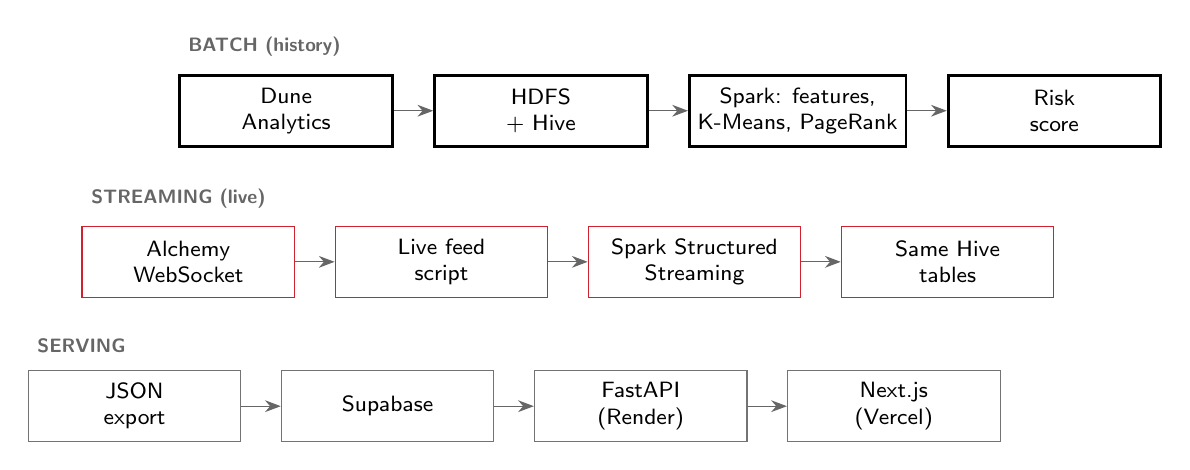
\begin{tikzpicture}[
  node distance=5mm,
  box/.style={draw,minimum height=9mm,minimum width=27mm,align=center,font=\footnotesize,inner sep=3pt},
  batch/.style={box,line width=1pt},
  stream/.style={box,draw=accent},
  serve/.style={box,draw=black!55},
  arr/.style={-{Stealth[length=2mm]},black!60}]
\node[font=\scriptsize\bfseries,black!60,anchor=west] (l1) at (0,0) {BATCH (history)};
\node[batch,below=1mm of l1.south west,anchor=north west] (b1) {Dune\\Analytics};
\node[batch,right=of b1] (b2) {HDFS\\+ Hive};
\node[batch,right=of b2] (b3) {Spark: features,\\K-Means, PageRank};
\node[batch,right=of b3] (b4) {Risk\\score};
\draw[arr] (b1)--(b2); \draw[arr] (b2)--(b3); \draw[arr] (b3)--(b4);

\node[font=\scriptsize\bfseries,black!60,anchor=west,below=4mm of b1.south west] (l2) {STREAMING (live)};
\node[stream,below=1mm of l2.south west,anchor=north west] (s1) {Alchemy\\WebSocket};
\node[stream,right=of s1] (s2) {Live feed\\script};
\node[stream,right=of s2] (s3) {Spark Structured\\Streaming};
\node[stream,right=of s3] (s4) {Same Hive\\tables};
\draw[arr] (s1)--(s2); \draw[arr] (s2)--(s3); \draw[arr] (s3)--(s4);

\node[font=\scriptsize\bfseries,black!60,anchor=west,below=4mm of s1.south west] (l3) {SERVING};
\node[serve,below=1mm of l3.south west,anchor=north west] (v1) {JSON\\export};
\node[serve,right=of v1] (v2) {Supabase};
\node[serve,right=of v2] (v3) {FastAPI\\(Render)};
\node[serve,right=of v3] (v4) {Next.js\\(Vercel)};
\draw[arr] (v1)--(v2); \draw[arr] (v2)--(v3); \draw[arr] (v3)--(v4);
\end{tikzpicture}
\caption*{Pipeline: batch and streaming paths meet in the same Hive tables, then are exported to the dashboard.}
\end{figure}

\section*{Tech Stack}
\begin{tabularx}{\linewidth}{@{}>{\raggedright\arraybackslash}p{3.2cm}X@{}}
\toprule
\textbf{Layer} & \textbf{Technology}\\
\midrule
Storage \& processing & \textbf{Hadoop 3.4.3} (HDFS, YARN, MapReduce), \textbf{Hive 3.1.3} (JDK 8), \textbf{Sqoop 1.4.7}\\
Compute \& ML & \textbf{Spark 3.5.5} (JDK 11): batch jobs, MLlib K-Means, logistic regression, random forest, GraphX PageRank, Structured Streaming\\
Ingestion & Python, Dune Analytics (historical), Alchemy WebSocket with \code{eth\_getLogs} gap-fill, CoinGecko prices; \code{systemd --user} keeps the live feed running\\
Live backend & Supabase (Postgres, row-level security), FastAPI on Render\\
Frontend & \textbf{Next.js 16} (App Router, Server Components), React 19, Tailwind CSS 4, IBM Plex fonts, hand-built SVG charts; hosted on Vercel\\
GenAI & Groq-hosted LLM for risk advisories and a grounded assistant (answers checked against tool output)\\
\bottomrule
\end{tabularx}

\section*{Features}
\begin{itemize}
\item One 0--100 stress score per pool pair, with a calm-to-crisis reference scale on every reading
\item Live-now cards and a live price chart updated from the streaming pipeline
\item Recent-activity panel: raw swaps with time windows and pair / pool / source filters
\item Two real case studies on one price axis: USDC recovered, UST did not
\item Evaluation page: lead time, false alarms, peak score, volume ratio, recovery
\item Leave-one-coin-out classifier comparison against the rule-based baseline, reported in both directions
\item PageRank wallet rankings with on-chain contract-vs-EOA checks
\item Frozen models and clear live-vs-frozen labelling, so no result is silently re-fitted
\end{itemize}

\section*{Screenshots}
\emph{Captured from the deployed site, \url{https://meridian-bda.vercel.app/} (data export of 1 Nov 2026).}

\shot{s_live.png}{Live now --- current risk scores and live price, streamed from Ethereum}
\shot{s_activity.png}{Recent activity --- raw swaps observed by the live feed}
\shot{s_risk.png}{Risk score per pair, and the USDC vs UST case studies on one axis}
\shot{s_class.png}{Classifier comparison --- trained on one coin, tested on the other}
\shot{s_wallet.png}{Wallet rankings --- most ``influential'' addresses are infrastructure, not traders}
\shot{s_eval.png}{Evaluation --- lead time, false alarms and recovery for both crises}

\section*{Results}
\begin{tabularx}{\linewidth}{@{}>{\raggedright\arraybackslash}p{4.2cm}X@{}}
\toprule
\textbf{Question} & \textbf{Result}\\
\midrule
Early warning, USDC (Mar 2023) & \textbf{72\,h} lead time before a sustained 1\% depeg (11.9\% max, low \$0.8808); peak score 81.2; elevated threshold 7.18; 12 brief false alarms over $\sim$6 months\\
Early warning, UST (May 2022) & \textbf{0\,h}. Data starts 15 Apr 2022, when UST was already unstable, so there is no ``before'' to measure. Peak 56.3; 34 false alarms with the USDC threshold. Reported, not hidden\\
Classifier, trained USDC $\rightarrow$ tested UST & Beats the rule baseline: F1 0.915 vs 0.858\\
Classifier, trained UST $\rightarrow$ tested USDC & Loses: F1 0.523 (logistic) / 0.611 (random forest) vs 0.995 for the rule\\
PageRank wallets & 19 of the top 20 addresses shown are contracts (routers, aggregators), checked against on-chain bytecode\\
Grounded GenAI assistant & 40 of 47 frozen test questions correct (85\%) after fixes, 36 of 47 (77\%) before; the grounding check caught 117 of 122 deliberately altered numbers\\
\bottomrule
\end{tabularx}

\section*{Limitations \& Honest Findings}
\begin{tabularx}{\linewidth}{@{}>{\raggedright\arraybackslash}p{4.4cm}X@{}}
\toprule
\textbf{Issue} & \textbf{How it is handled}\\
\midrule
Only two historical events & Presented as evidence for those events, not a general predictor. Not financial advice\\
UST has no calm baseline & Its pools were unstable before the crisis window; UST is reported separately and never pooled with USDC\\
Hive is slow (46--56\,s for a trivial \code{COUNT(*)} on MapReduce) & The dashboard never queries Hive; a Spark export materialises JSON that is pushed to Supabase\\
Re-fitting would invalidate published results & Frozen model artifacts; streaming uses \code{.transform()} only\\
Live price spikes (e.g.\ USDC\_DAI) & Hourly price is a plain average of per-swap ratios, so dust-volume hours (under \$1 traded) can spike it. A volume-weighted price would remove this\\
Live wallet concentration is a constant & Live rows use the USDC-calm value (0.1283); volume anomaly is not exported per live row\\
``Live now'' freshness & Scores are only as fresh as the last Spark export and push to Supabase\\
\bottomrule
\end{tabularx}

\section*{Running It}
\begin{minipage}{\linewidth}\begin{lstlisting}
# dashboard (RENDER_API_URL must point at the FastAPI backend)
cd dashboard
npm ci
npm run dev            # http://localhost:3000

# pipeline: needs the local Hadoop / Hive / Spark stack, see docs/SETUP.md
# 1. run spark/export_dashboard_data.scala   (writes dashboard/data/*.json)
# 2. python ingestion/push_to_supabase.py    (pushes the JSON to Supabase)
\end{lstlisting}\end{minipage}

\section*{Repository Layout}
\begin{tabularx}{\linewidth}{@{}>{\raggedright\arraybackslash}p{4.4cm}X@{}}
\toprule
\textbf{Path} & \textbf{Contents}\\
\midrule
\code{ingestion/} & Historical backfill and live Alchemy feed\\
\code{hive/} & Hive DDL\\
\code{spark/} & Batch jobs, ML, PageRank, dashboard export, streaming consumer\\
\code{dashboard/} & Next.js dashboard (Vercel)\\
\code{backend/} & FastAPI service (Render), grounded assistant\\
\code{supabase/}, \code{systemd/}, \code{genai/}, \code{docs/} & Schema, always-on services, GenAI evaluation, full documentation\\
\bottomrule
\end{tabularx}

\end{document}
